

For searches characterized by such limited statistics, maximizing the cut position through a purely systematic approach that maximizes the significance of the excess is a double-edged sword. On one hand, it certainly helps identify patterns, structures, and correlations among the cuts but, on the other hand, it carries the risk of overfitting the very limited data.

To extract the best possible values given the available dataset, an MCMC method was applied to sample the 10-dimensional space of cut positions, optimizing the significance computed with Eq.~\ref{eq:basic_formula}. During the optimization, two artificial constraints are imposed:
\begin{itemize}
\item \textbf{Minimum 3 neutrino events per hour}: although better signal-over-background ratios might in principle be achieved by removing even more events, the limited size of the available datasets makes it safer to require a minimum expected event rate.
\item \textbf{Minimum 5 background events in total}: below this threshold, the optimization loses meaning, as the absolute number of events becomes too small.
\end{itemize}
% ------------------------------------------------------------
% Table 1: Optimized cut values
% ------------------------------------------------------------
\begin{table}[htbp]
    \centering
    \begin{tabular}{lcc}
        \hline
        Cut variable & Default value & Optimized value \\
        \hline
        Vertex fiducial volume ($z$-coordinate)   & 20      & 17.55   \\
        Vertex fiducial volume ($y$-coordinate)   & 550     & 416.96  \\
        N daughter particles                      & 6       & 7    \\
        Max $\cos(\theta_{\mathrm{beam}})$         & 0.970   & 0.965   \\
        Cut on $C_{0-10}$                          & 3000    & 1224.28 \\
        Cut on $C_{40-50}$                          & 10000   & 3372.87 \\
        Cut on $C_{140-150}$                        & 3000    & 3194.63 \\
        ROI Z size                                 & 15      & 23.40   \\
        ROI Z close to vertex                      & 20      & 30.32   \\
        Tail Length Density                        & 0.200   & 0.440   \\
        \hline
    \end{tabular}
    \caption{Optimized cut values obtained from the MCMC significance maximization.}
    \label{tab:best_parameters_v1}
\end{table}

% ------------------------------------------------------------
% Table 2: Event yields and performance metrics after cuts
% ------------------------------------------------------------
\begin{table}[htbp]
    \centering
    \begin{tabular}{lcc}
        \hline
        Quantity & Default cuts & Optimized cuts \\
        \hline
        MC events after cuts (normalized)                  & 2.91   & 3.08   \\
        Off-spill data events after cuts (normalized)      & 0.448  & 0.224  \\
        MC / off-spill data ratio (normalized)             & 6.51   & 13.77  \\
        Efficiency                                         & 0.143  & 0.151  \\
        Purity                                             & 0.867  & 0.932  \\
        F1 score                                           & 0.246  & 0.260  \\
        Significance                                       & 127.75 & 192.28 \\
        MC events after cuts (absolute)                    & 1732   & 1831   \\
        Off-spill data events after cuts (absolute)        & 20     & 10     \\
        \hline
    \end{tabular}
    \caption{Event yields and performance metrics after applying the optimized cuts.}
    \label{tab:results_summary_v1}
\end{table}



A comparison between the hand-chosen and best combination of values for the cuts is reported in Tab. \ref{tab:best_parameters_v1}. Among these, the maximum Y cut on the vertex position changes significantly, with the optimized cut removing ~2 meters from the top. This is consistent with neutrinos being expected to interact more often in the lower section of the detector.

The performance metrics are reported in Tab. \ref{tab:results_summary_v1}, where a clear improvement is visible in all the considered metrics. Moreover, each variable has been tested by plotting the evolution of the considered metrics at the change of the cut position, fixing every other cut to its best position (Fig. \ref{fig:direction_z_max_v1}-\ref{fig:vertex_z_min_v1}). 



% ------------------------------------------------------------
% Figures: one figure per cut variable, stacking the
% score/efficiency/purity/significance plot and the total
% events plot.
% ------------------------------------------------------------
\begin{figure}[h]
    \centering
    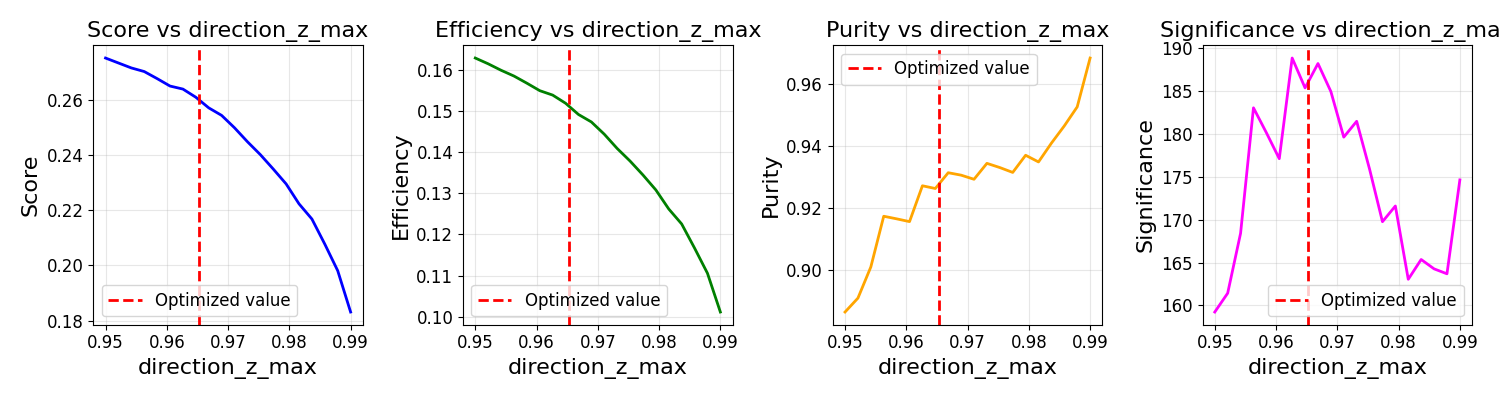
\includegraphics[width=0.69\linewidth]{sections/plots/version_1/cut_optimization/direction_z_max_score_efficiency_purity_significance.png}\\
    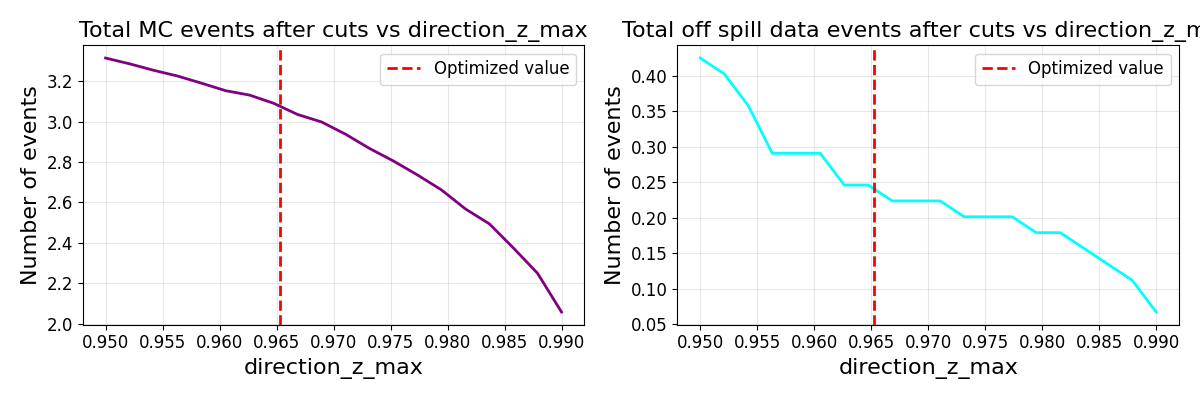
\includegraphics[width=0.69\linewidth]{sections/plots/version_1/cut_optimization/direction_z_max_total_events.png}
    \caption{Score, efficiency, purity, significance, and total number of MC and off-spill data events surviving the selection as a function of the cut on Max $\cos(\theta_{\mathrm{beam}})$. The red dashed line indicates the optimized cut value.}
    \label{fig:direction_z_max_v1}
\end{figure}
\begin{figure}[h]
    \centering
    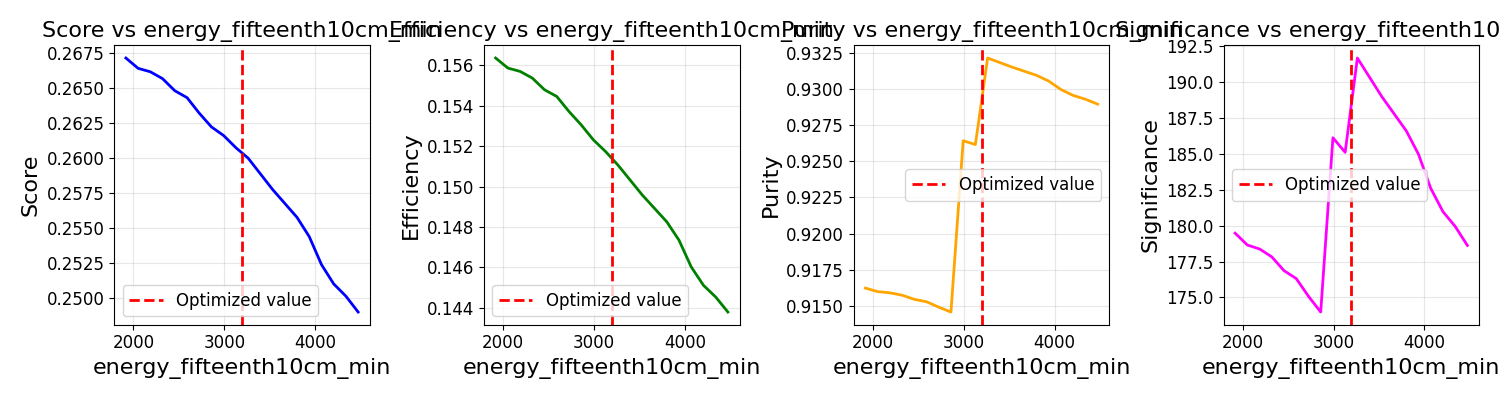
\includegraphics[width=0.69\linewidth]{sections/plots/version_1/cut_optimization/energy_fifteenth10cm_min_score_efficiency_purity_significance.png}\\
    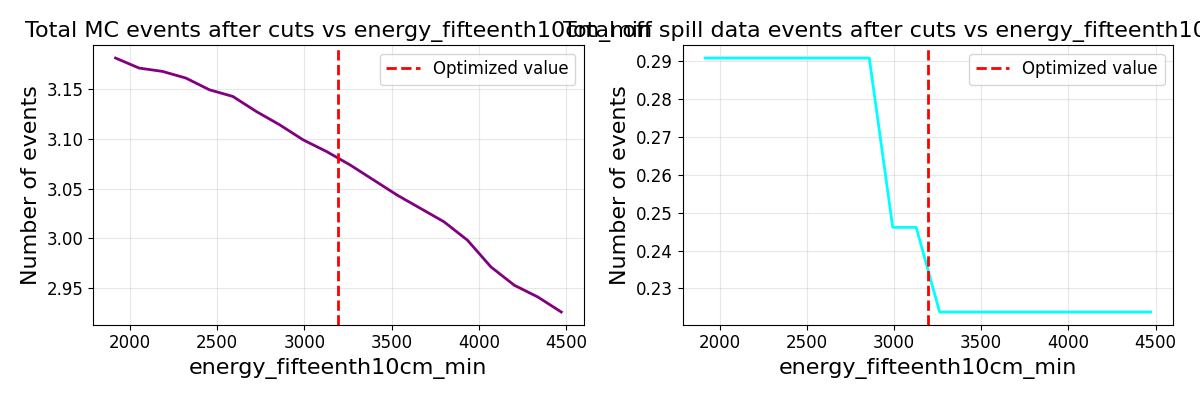
\includegraphics[width=0.69\linewidth]{sections/plots/version_1/cut_optimization/energy_fifteenth10cm_min_total_events.png}
    \caption{Score, efficiency, purity, significance, and total number of MC and off-spill data events surviving the selection as a function of the cut on $C_{140-150}$. The red dashed line indicates the optimized cut value.}
    \label{fig:energy_fifteenth10cm_min_v1}
\end{figure}
\begin{figure}[h]
    \centering
    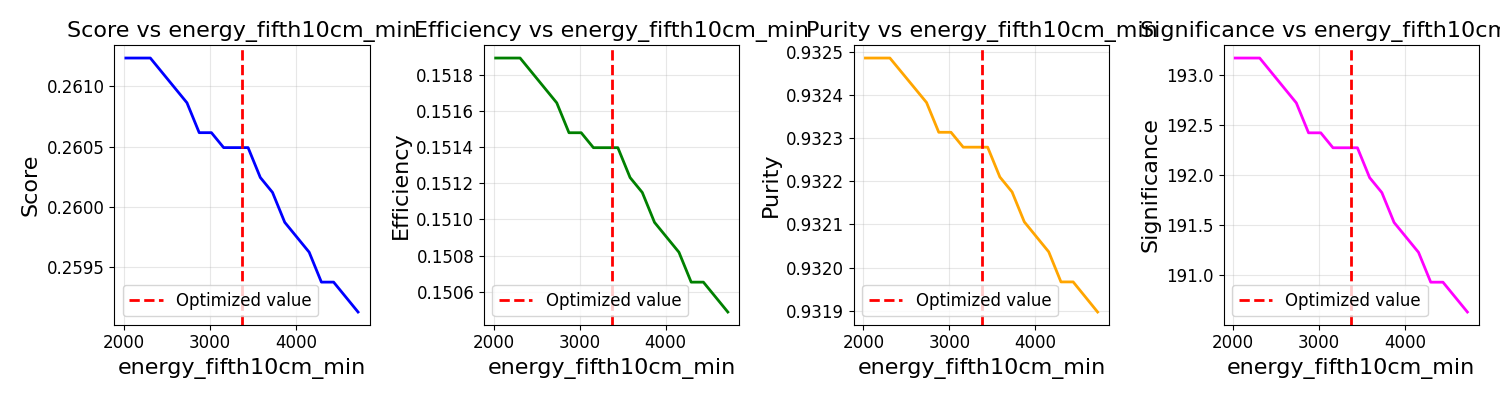
\includegraphics[width=0.69\linewidth]{sections/plots/version_1/cut_optimization/energy_fifth10cm_min_score_efficiency_purity_significance.png}\\
    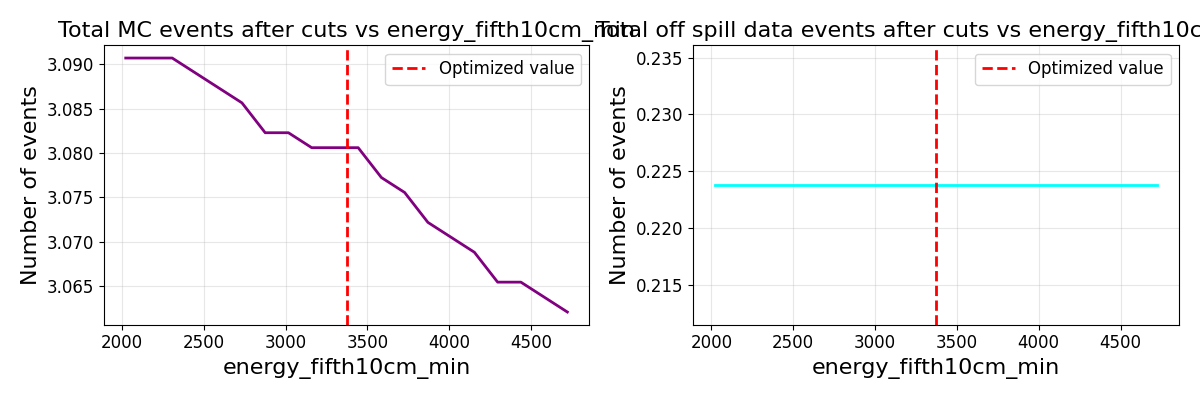
\includegraphics[width=0.69\linewidth]{sections/plots/version_1/cut_optimization/energy_fifth10cm_min_total_events.png}
    \caption{Score, efficiency, purity, significance, and total number of MC and off-spill data events surviving the selection as a function of the cut on $C_{40-50}$. The red dashed line indicates the optimized cut value.}
    \label{fig:energy_fifth10cm_min_v1}
\end{figure}
\begin{figure}[h]
    \centering
    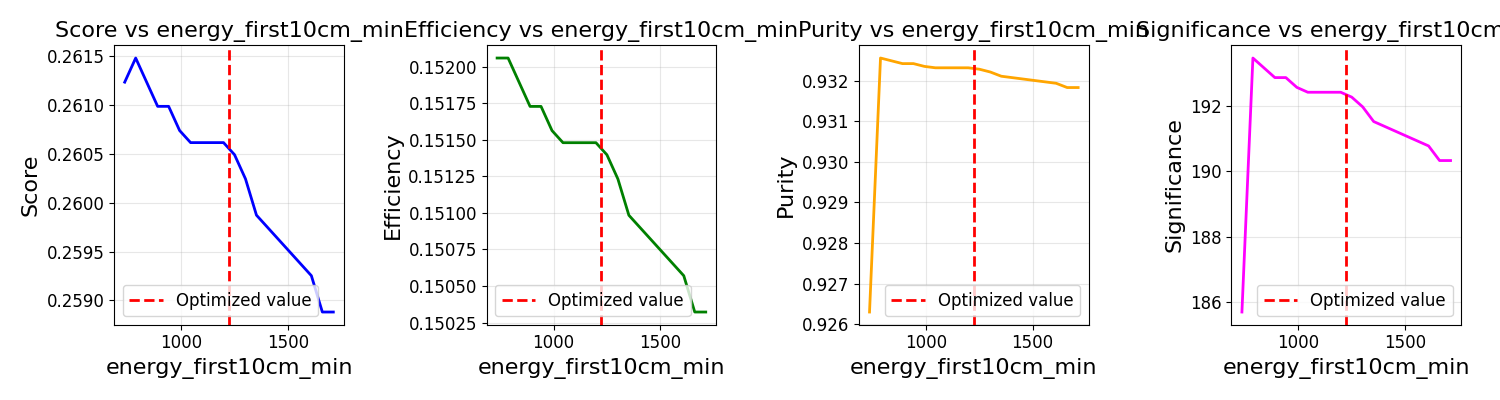
\includegraphics[width=0.69\linewidth]{sections/plots/version_1/cut_optimization/energy_first10cm_min_score_efficiency_purity_significance.png}\\
    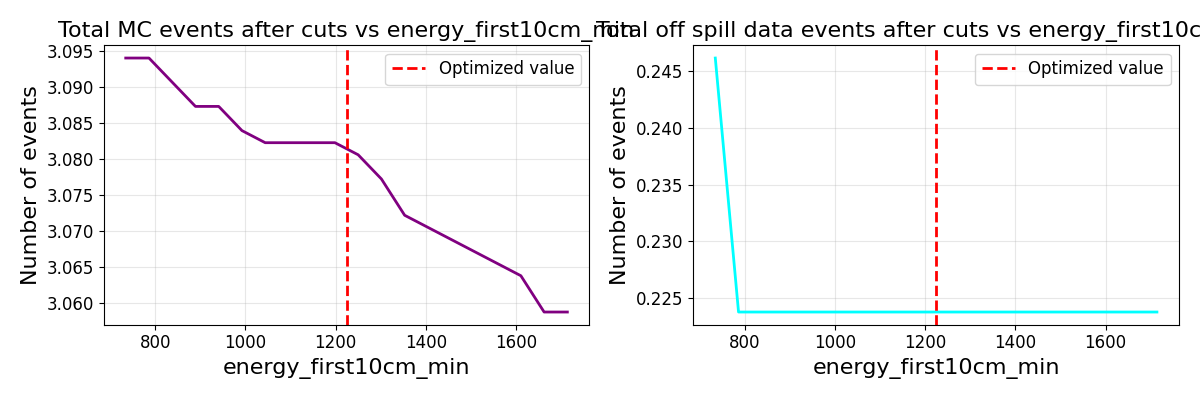
\includegraphics[width=0.69\linewidth]{sections/plots/version_1/cut_optimization/energy_first10cm_min_total_events.png}
    \caption{Score, efficiency, purity, significance, and total number of MC and off-spill data events surviving the selection as a function of the cut on $C_{0-10}$. The red dashed line indicates the optimized cut value.}
    \label{fig:energy_first10cm_min_v1}
\end{figure}
\begin{figure}[h]
    \centering
    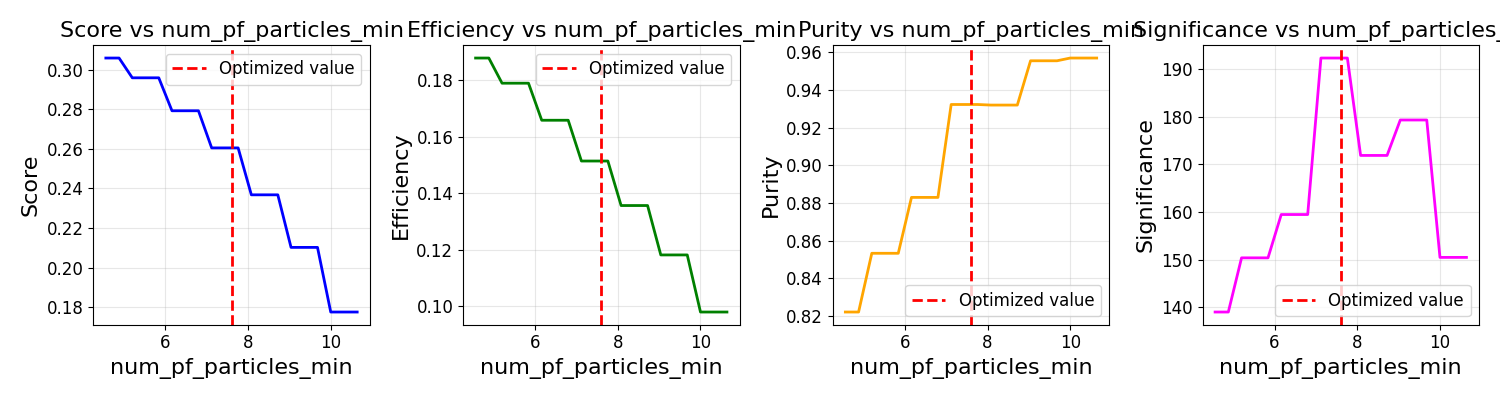
\includegraphics[width=0.69\linewidth]{sections/plots/version_1/cut_optimization/num_pf_particles_min_score_efficiency_purity_significance.png}\\
    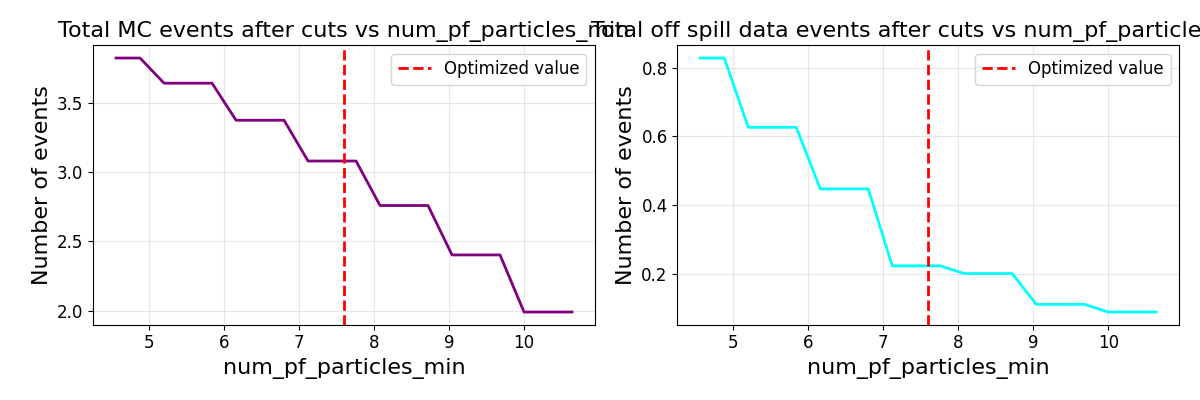
\includegraphics[width=0.69\linewidth]{sections/plots/version_1/cut_optimization/num_pf_particles_min_total_events.png}
    \caption{Score, efficiency, purity, significance, and total number of MC and off-spill data events surviving the selection as a function of the cut on N daughter particles. The red dashed line indicates the optimized cut value.}
    \label{fig:num_pf_particles_min_v1}
\end{figure}
\begin{figure}[h]
    \centering
    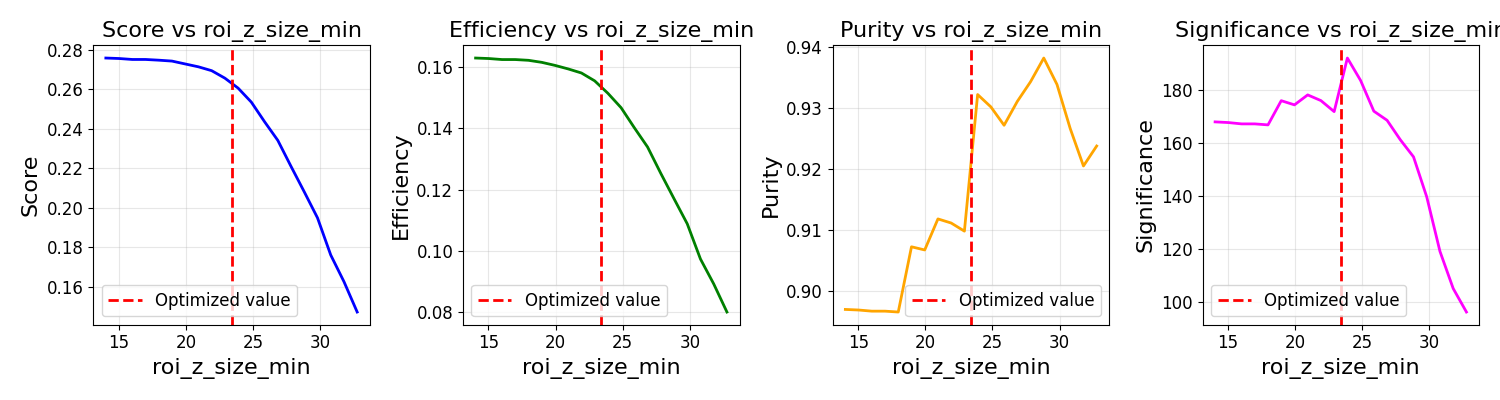
\includegraphics[width=0.69\linewidth]{sections/plots/version_1/cut_optimization/roi_z_size_min_score_efficiency_purity_significance.png}\\
    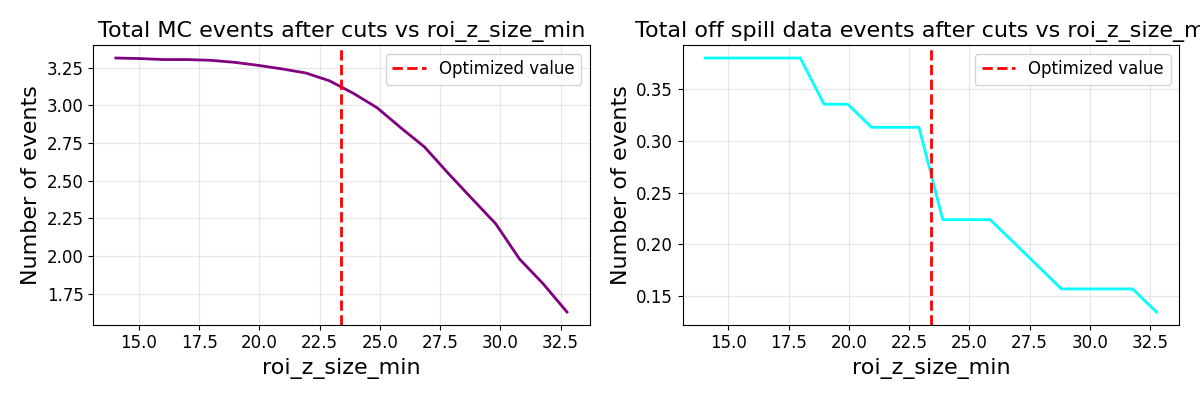
\includegraphics[width=0.69\linewidth]{sections/plots/version_1/cut_optimization/roi_z_size_min_total_events.png}
    \caption{Score, efficiency, purity, significance, and total number of MC and off-spill data events surviving the selection as a function of the cut on ROI Z size. The red dashed line indicates the optimized cut value.}
    \label{fig:roi_z_size_min_v1}
\end{figure}
\begin{figure}[h]
    \centering
    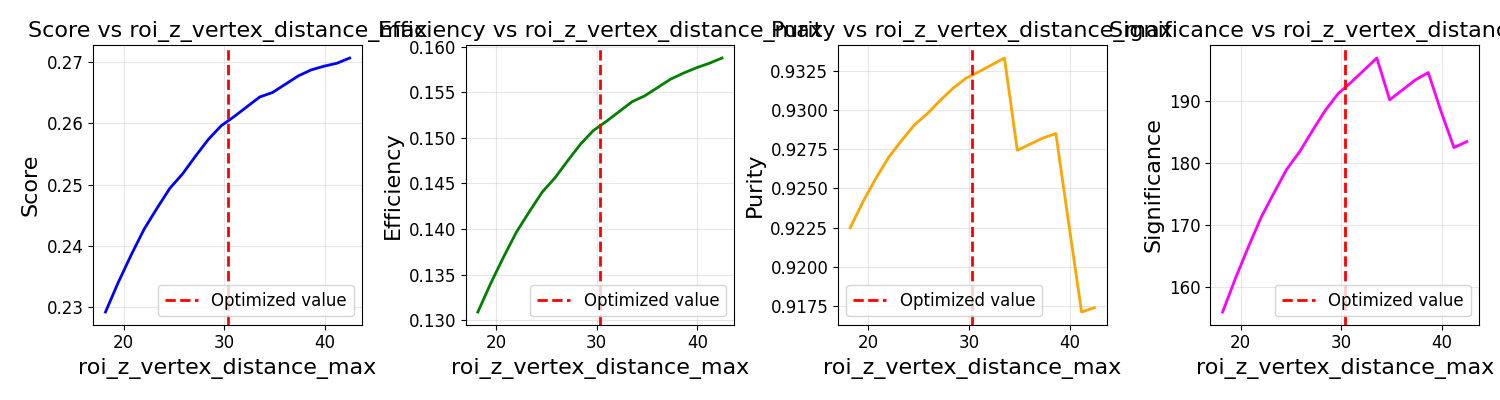
\includegraphics[width=0.69\linewidth]{sections/plots/version_1/cut_optimization/roi_z_vertex_distance_max_score_efficiency_purity_significance.png}\\
    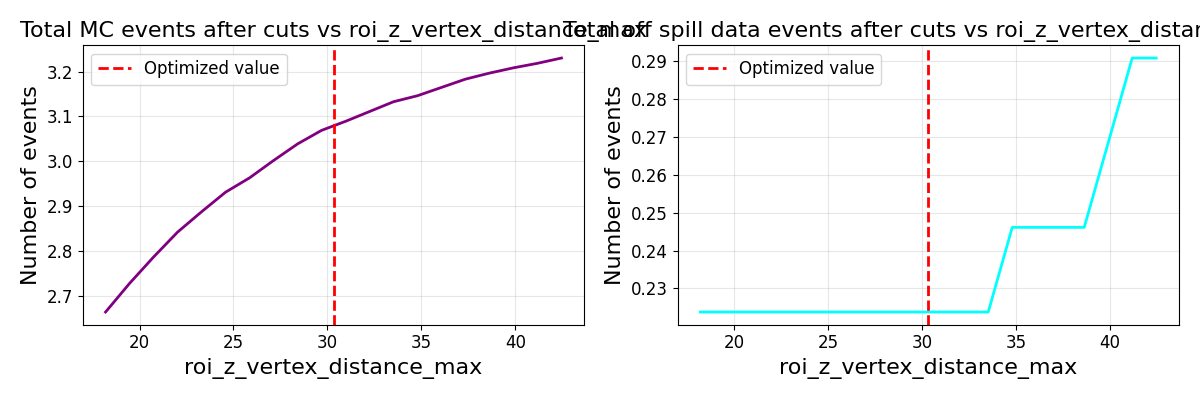
\includegraphics[width=0.69\linewidth]{sections/plots/version_1/cut_optimization/roi_z_vertex_distance_max_total_events.png}
    \caption{Score, efficiency, purity, significance, and total number of MC and off-spill data events surviving the selection as a function of the cut on ROI Z close to vertex. The red dashed line indicates the optimized cut value.}
    \label{fig:roi_z_vertex_distance_max_v1}
\end{figure}
\begin{figure}[h]
    \centering
    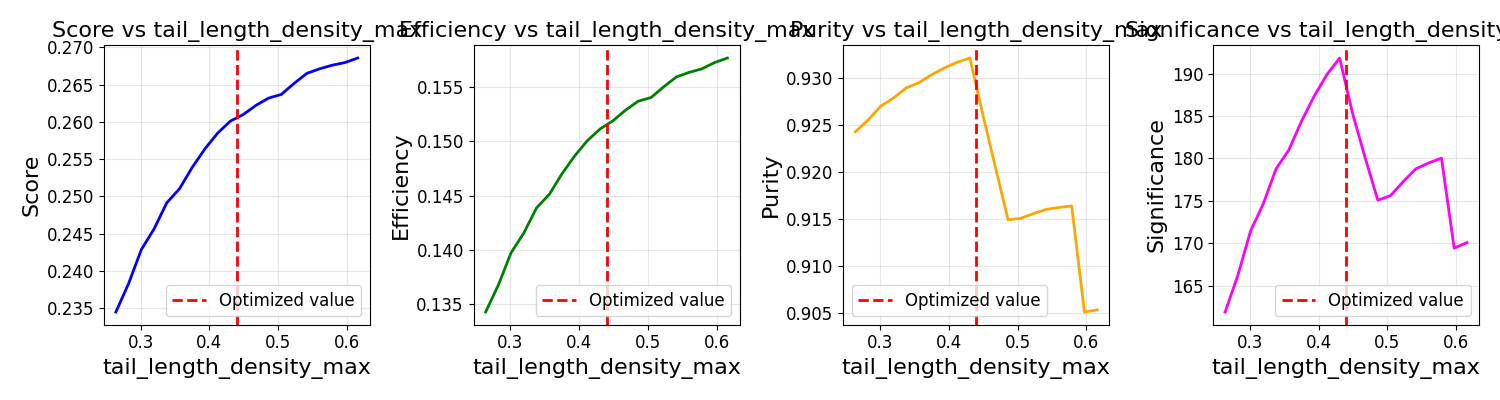
\includegraphics[width=0.69\linewidth]{sections/plots/version_1/cut_optimization/tail_length_density_max_score_efficiency_purity_significance.png}\\
    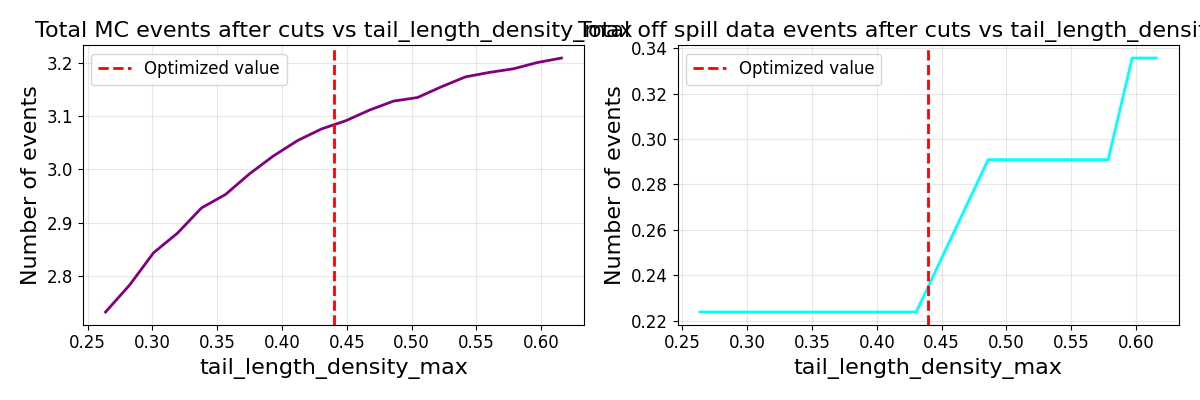
\includegraphics[width=0.69\linewidth]{sections/plots/version_1/cut_optimization/tail_length_density_max_total_events.png}
    \caption{Score, efficiency, purity, significance, and total number of MC and off-spill data events surviving the selection as a function of the cut on Tail Length Density. The red dashed line indicates the optimized cut value.}
    \label{fig:tail_length_density_max_v1}
\end{figure}
\begin{figure}[h]
    \centering
    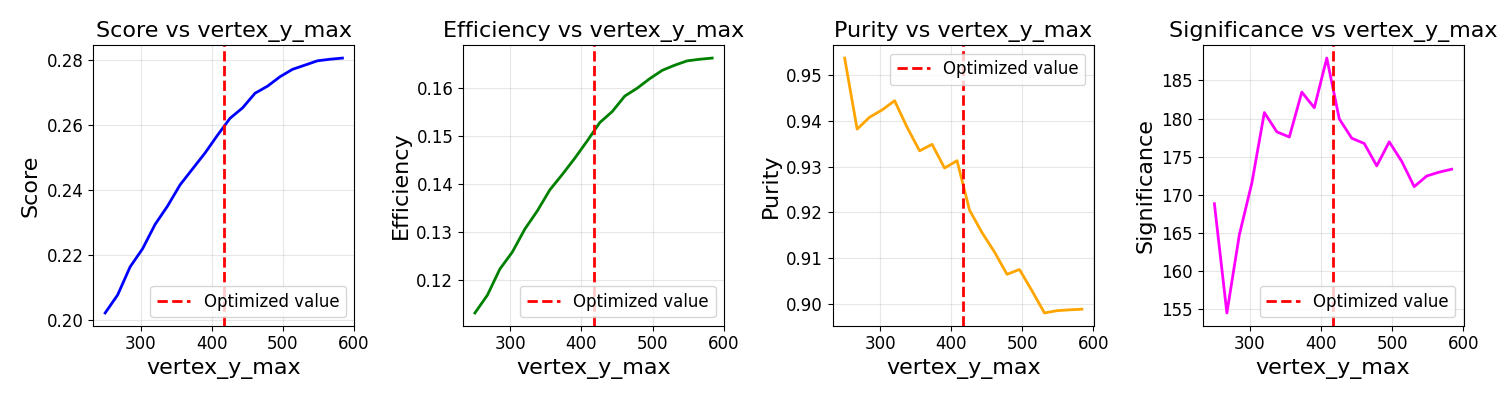
\includegraphics[width=0.69\linewidth]{sections/plots/version_1/cut_optimization/vertex_y_max_score_efficiency_purity_significance.png}\\
    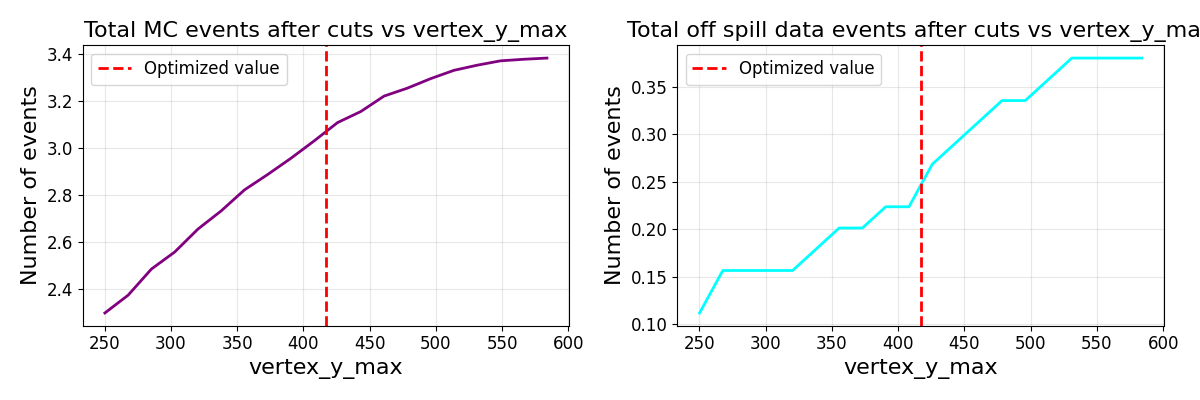
\includegraphics[width=0.69\linewidth]{sections/plots/version_1/cut_optimization/vertex_y_max_total_events.png}
    \caption{Score, efficiency, purity, significance, and total number of MC and off-spill data events surviving the selection as a function of the cut on Vertex fiducial volume ($y$-coordinate). The red dashed line indicates the optimized cut value.}
    \label{fig:vertex_y_max_v1}
\end{figure}
\begin{figure}[h]
    \centering
    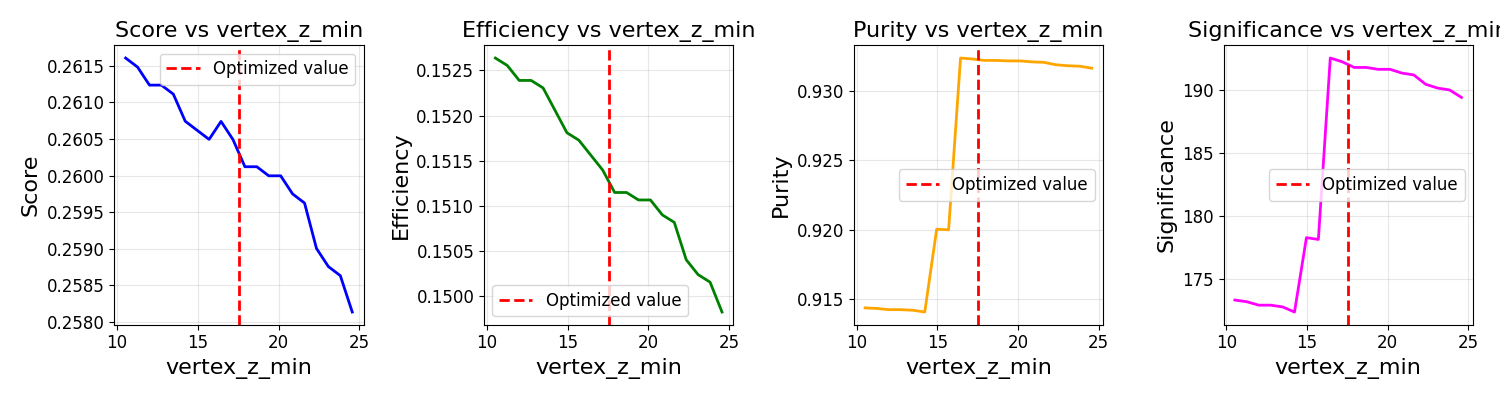
\includegraphics[width=0.69\linewidth]{sections/plots/version_1/cut_optimization/vertex_z_min_score_efficiency_purity_significance.png}\\
    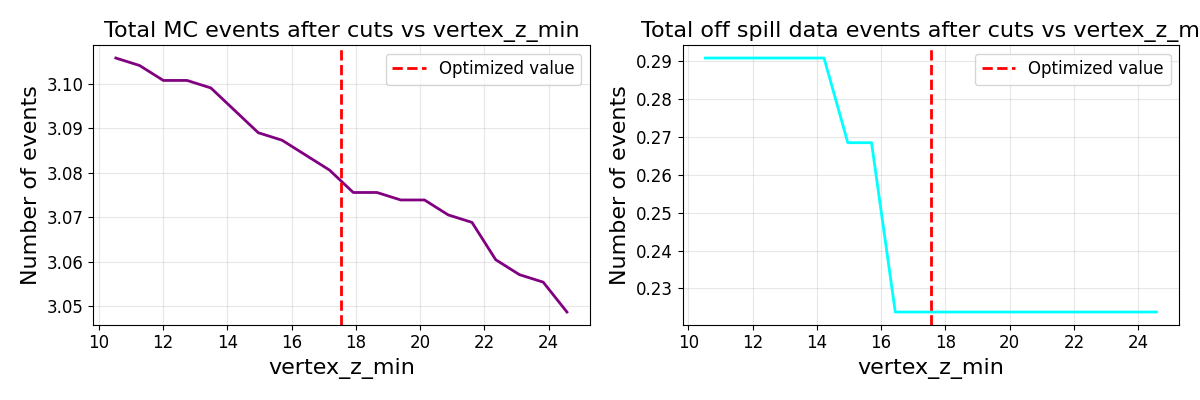
\includegraphics[width=0.69\linewidth]{sections/plots/version_1/cut_optimization/vertex_z_min_total_events.png}
    \caption{Score, efficiency, purity, significance, and total number of MC and off-spill data events surviving the selection as a function of the cut on Vertex fiducial volume ($z$-coordinate). The red dashed line indicates the optimized cut value.}
    \label{fig:vertex_z_min_v1}
\end{figure}

